
\documentclass{article}

\usepackage[left=1.8cm,right=1.8cm, top=2cm, bottom = 2cm]{geometry}
\usepackage{amsfonts}

\usepackage{amsmath}
\usepackage{xcolor}

\usepackage{tikz}
\usepackage{subfigure}

\usepackage{pgfplots}

\pgfplotsset{compat=1.10}
\usepgfplotslibrary{fillbetween}
\usetikzlibrary{patterns}



\pagestyle{empty}

\setlength{\tabcolsep}{15pt}


\newcommand{\deriv}[3][]{\frac{\mathrm{d}^{#1}#2}{\mathrm{d}#3^{#1}}}
\newcommand{\diff}{\;\mathrm{d}}

\newcommand{\norm}[1]{\left|\kern-1pt\left|#1\right|\kern-1pt\right|}
\newcommand{\bra}[1]{\left\langle #1 \,\right|}
\newcommand{\ket}[1]{\left|\, #1\right\rangle}
\newcommand{\braket}[2]{\left\langle #1 \mid #2 \right\rangle}




\begin{document}

\title{Bode Plots}
\date{}

\maketitle
\thispagestyle{empty}

\Large

\vskip -10mm

\textbf{\underline{Objective: To sketch Bode plots and estimate gain and phase margins.}}



\vspace{5mm}



\textbf{Recap: Fourier and Laplace Transforms:}\bigskip

Recall that, given a function $f(t)$ on the time-domain, the (angular-frequency) Fourier transform is
\[\hat{f}(\omega)=\int_{-\infty}^\infty f(t)e^{-j\omega t}\diff t,\]
while the Laplace transform is
\[\mathcal{L}(f)(s)=\int_0^\infty f(t)e^{-st}\diff t.\]


\begin{enumerate}
	\item Suppose that $f(t)=0$ for all $t<0$. Show that, when $s=j\omega$,
		\[\mathcal{L}(f)(j\omega)=\hat{f}(\omega).\]
	\item Suppose $f(t)$ has Laplace transform
		\[F(s)=\frac{e^{-7s}}{s(s-1)}.\]
		Write down the Fourier transform $\hat{f}(\omega)$.
\end{enumerate}







\clearpage


\textbf{Theory: The Laplace and Frequency Domains:}\bigskip



Recall that the Fourier transform of a function tells us what combination of frequencies produces that function. That is, if we imagine a note of each different frequency $\omega$, each playing with amplitude given by $\hat{f}(\omega)$, then the superposition of those notes (the sound formed by them interfering with each other) would be the function $f(t)$.

The Laplace transform generalises this by introuducing an exponential decay (or growth!) rate $\sigma$. For a complex number $s=\sigma+\omega j$, we have
\begin{align*}
	e^{st}&=e^{\sigma t + j\omega t}\\
	&=e^{\sigma t}e^{j\omega t},
\end{align*}
a complex sinusoid with (angular) frequency $\omega$, growing exponentially at rate $\sigma$ (or decaying, if $\sigma<0$). So for the Laplace transform of $f(t)$, imagine a note playing at frequency $\omega$, with initial amplitude $\mathcal{L}(f)(\sigma +j\omega)$ and decaying exponentially with rate $\sigma$; if you fix $\sigma$ and take every different note in this way, their superposition will be the original function $f(t)$ (by Mellin's inverse formula).

So the Laplace transform tells us for each different decay rate $\mathrm{re}(s)$, what amplitude $\mathcal{L}(f)(\sigma+j\omega)$ to assign to each note of frequency $\omega$ to produce a particular function when all these notes combine. As such, the Laplace domain (where the variable $s$ lives) is the complex plane, where real part can be thought of as a decay rate and imaginary part as a frequency. Within the complex plane is the imaginary axis, where $\mathrm{re}(s)=0$, and this can be thought of as the frequency domain (where the variable $\omega$ lives). If we restrict the Laplace transform by only looking at what happens when $\mathrm{re}(s)=0$, then we get the Fourier transform (at least for functions which are 0 for negative times).\bigskip


Now consider an LTI system with transfer function $T(s)$. The \textbf{frequency response} of the system is $T(j\omega)$, the restriction of the transfer function to the imaginary axis. Since the transfer function is the Laplace transform of the impulse response, the frequency response is simply the Fourier transform of the impulse response. When a signal $f(t)$ is input into the system, its Laplace transform $F(s)$ is multiplied by the transfer function to give output $F(s)T(s)$. When restricting to the imaginary axis, we are looking at $\hat{f}(\omega)T(j\omega)$---so the frequency response $T(j\omega)$ is the amount we multiply $\hat{f}(\omega)$ by to get the output.

So we can think of the LTI as a frequency-dependent amplifier; $T(j\omega)$ is the amplifier's gain at frequency $\omega$. It is the amount you multiply the sinusoid of frequency $\omega$ by as it passes through the system.




\clearpage



\textbf{Complex Gain and Bode Plots:}\bigskip


We saw above that the frequency response (the restriction of the transfer function to the imaginary axis) tells us how much to amplify each frequency component of the input signal by to get the output. In particular, if we input a sinusoid $Ae^{j\omega t}$ to the LTI system, the output will be a sinusoid of the same frequency, $AT(j\omega)e^{j\omega t}$.

But $T(j\omega)$ could be a complex number, $T(j\omega) = re^{j\theta}$ in polar form, so the output is $Are^{j(\omega t+\theta)}$; the amplitude is scaled by $r$ (the modulus of $T(j\omega)$), and the sinusoid is phase shifted by $\theta$ (the argument of $T(j\omega)$). So when passing a sinusoid through the system, not only is its amplitude amplified, but it also experiences a phase shift.

Therefore to describe the frequency response of a system, we need to give two pieces of information: for each input frequency $\omega$, we need to give the gain on the amplitude (the modulus of $T(j\omega)$) and also the phase shift (the argument of $T(j\omega)$). This is conveniently done by the use of two plots: the \textbf{Bode gain plot} shows the amplitude gain (on the $y$-axis) at each frequency (on the $x$-axis); the \textbf{Bode phase plot} show the phase shift (on the $y$-axis) at each frequency (on the $x$-axis). These plots are typically displayed vertically aligned, so that it is easy to read off both the gain and phase at a given frequency.\bigskip


Give the outputs for a selection of sinusoidal inputs to the system with this Bode plot.
\begin{center}
	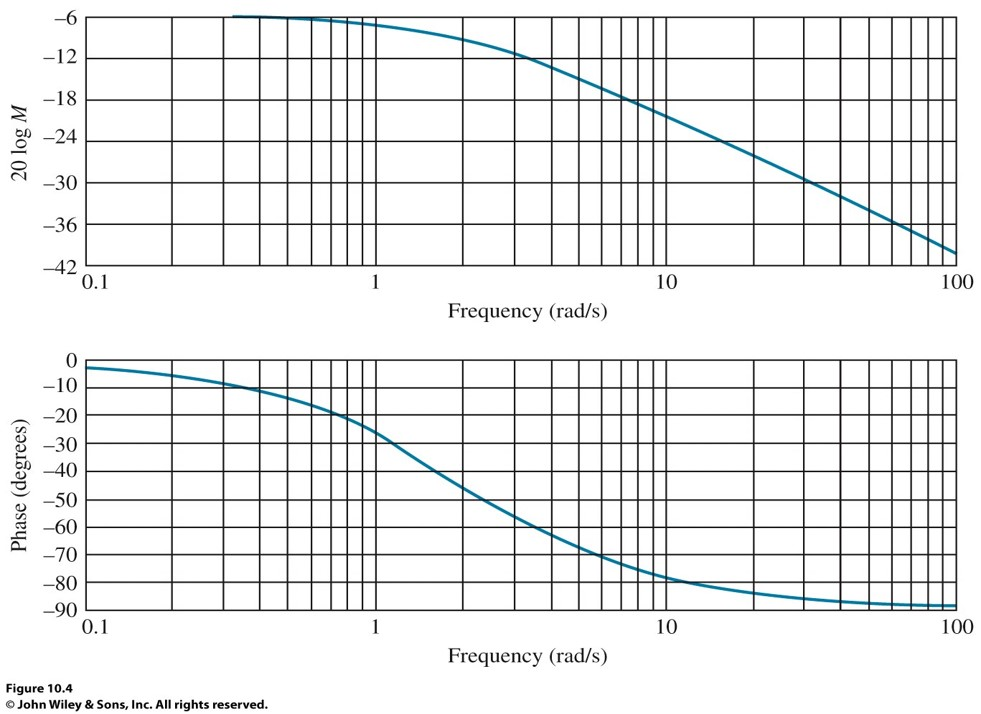
\includegraphics[scale=0.9]{BodeExample.jpg}
\end{center}


\clearpage



\textbf{Gain and Phase Margins:}\bigskip


Suppose we have an open-loop system with transfer function $T(s)$, and want to introduce negative feedback, with feedback gain $F(s)$. Will the resulting system still be stable?

Show that the overall transfer function of the system with feedback is
\[\frac{T(s)}{1+F(s)T(s)}.\]
\vfill

This will have a pole wherever $T(s)$ has a pole; but that would already cause instability in the original, open-loop system, so is not a new problem with the feedback. There will additionally be a new pole at any value of $s$ such that $1+F(s)T(s)=0$. So we are interested in whether or not $F(s)T(s)$ can ever equal $-1$. As a complex number, $-1$ has modulus 1 and argument $\pi$ (or $-\pi$, equivalently!). So we are interested in values of $s$ for which $|F(s)T(s)|=1$ or $\arg(F(s)T(s))=\pi$, and in particular whether both occur together!

If we draw a Bode plot for $F(s)T(s)$, then we can read off from the gain plot when $|F(s)T(s)|=1$, and from the phase plot when $\arg(F(s)T(s))=\pi$. If these occur at the same frequency $\omega$, then we know we will have a pole in the closed-loop system at that frequency.

We can look up from the phase plot at what frequency the phase is $\pi$; then the gain plot will tell us the gain $G$ at that frequency. We then have a ``margin of safety'' of $G$---we would need to reduce the gain by $G$ before an instability would occur. This is called the \textbf{gain margin}.

Similarly, we can look up the frequency at which the gain is 1, and then look on the phase plot to see how far from $\pi$ the phase is at that frequency; this gives us the \textbf{phase margin}, or how much we can increase the phase shift by before creating an instability in the closed-loop system.

\begin{center}
	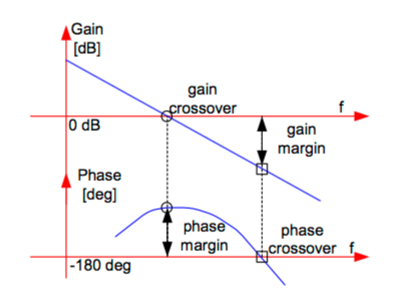
\includegraphics[scale=0.5]{BodeMargins.jpg}
\end{center}













\end{document}